\section{Visibilität}

\textit{Algorithmen für verdeckte Linien und Flächen}

\begin{itemize}
  \item Backface Culling
  \item Tiefensortierung
  \item Z-Buffer
  \item Warnock Algorithmus
  \item Raycasting / Raytracing
\end{itemize}

\subsection{Backface Culling (WebGL)}

\begin{itemize}
  \item Rückseiten nicht zeichnen
  \item Test durch Normalvektor (Normalvektor der Fläche Richtung Kamera, dann zeichnen)
\end{itemize}

\subsection{Tiefensortierung (Painters Algorithms)}

\textit{Zeichnen der Polygone in einer Reihenfolge zuletzt gezeichnete überdecken die ersten Sortierung}

Sortierung:
\begin{enumerate}
  \item Sortierung nach minmaler y-Koordinate (in Kamera Koordinaten)
  \item wenn in z-überlagern -> weitere Bedingungen beachten
  \item Falls keine Bedingung erfüllt -> Polygone vertauschen und nochmals Prüfen
\end{enumerate}

\textit{Wenn [P,Q] Reihenfolge, austauschen wenn KEINE der folgenden Bedingungen zutrifft}:\\

\begin{tabular}{cl}
  \multirow{3}{*}{
    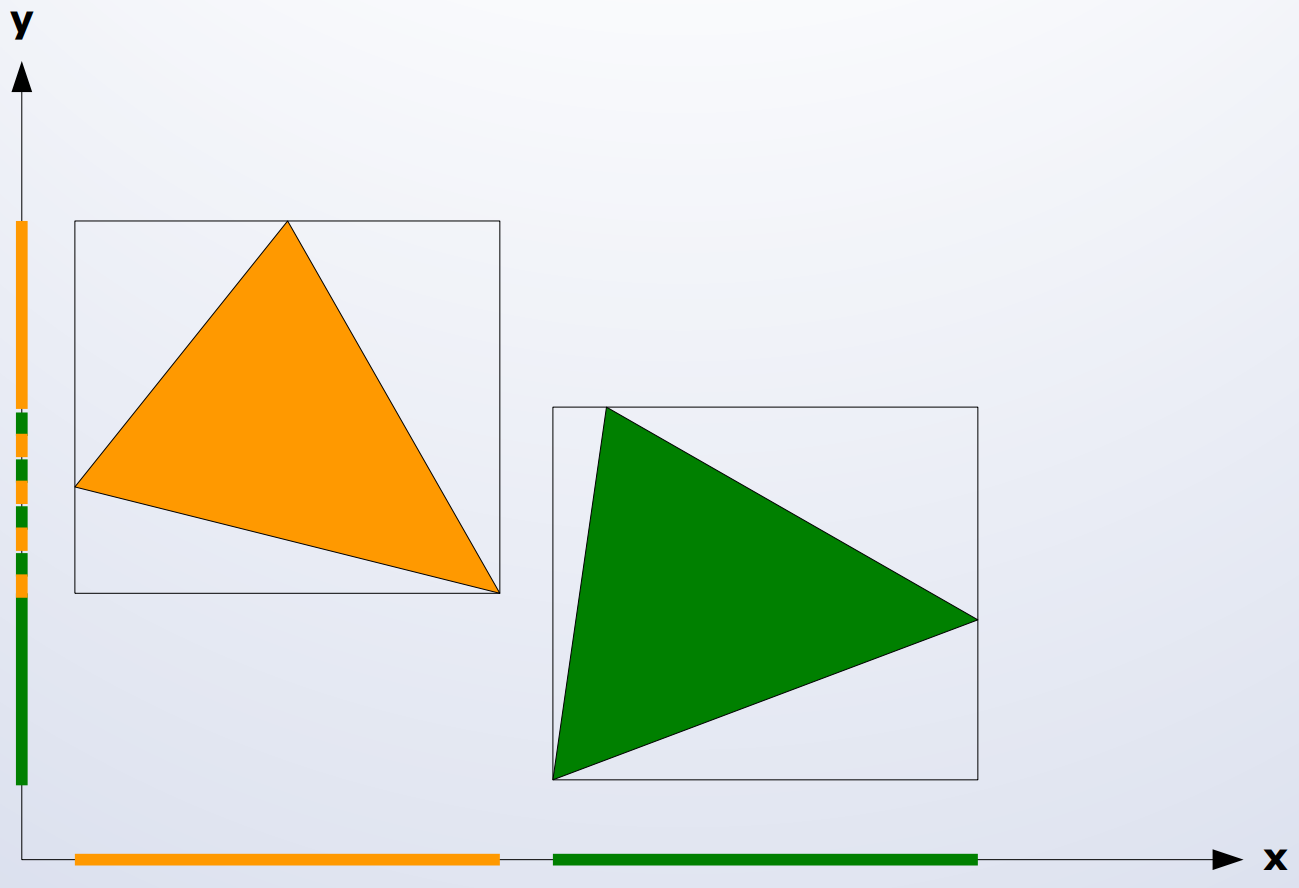
\includegraphics[width=0.25\textwidth]{assets/paintersalg-overlapping.png}
  } & 1. Überlagern sich die \\
  & x-Ausdehnungen nicht? \\
  & (vollständig nebeneinander) \\
  & \\
  & 2. Überlagern sich die \\
  & y-Ausdehnungen nicht? \\
  & (vollständing hintereinander)\\
\end{tabular}

\begin{tabular}{cl}
  \multirow{3}{*}{
    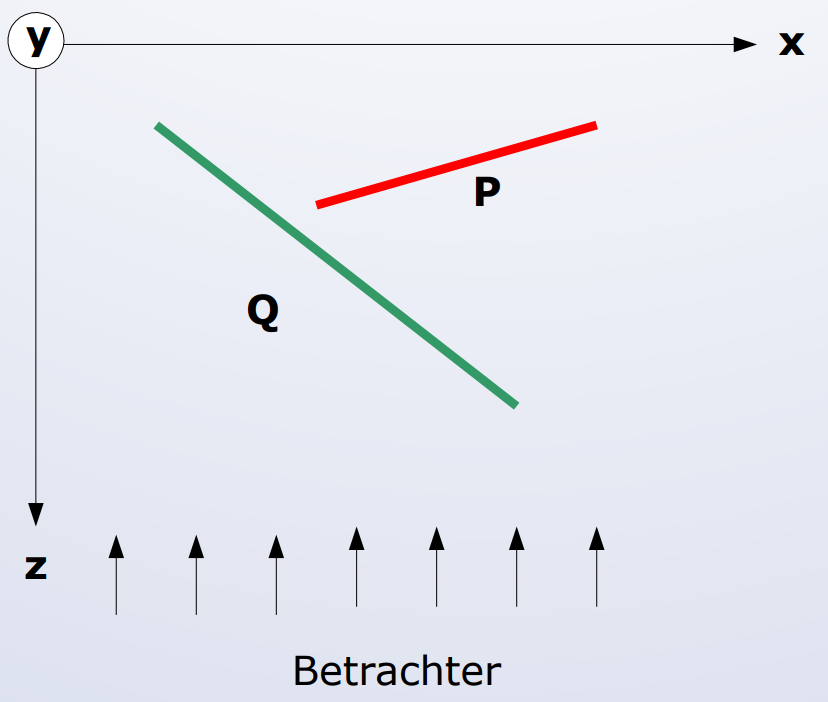
\includegraphics[width=0.15\textwidth]{assets/paintersalg-backside.png}
  } & \\
  & 3. Wird das hintere Objekt P vom \\
  & Vorderen Q komplett überdeckt? \\
  & \\
  & \\
  & \\
\end{tabular}

\begin{tabular}{cl}
  \multirow{3}{*}{
    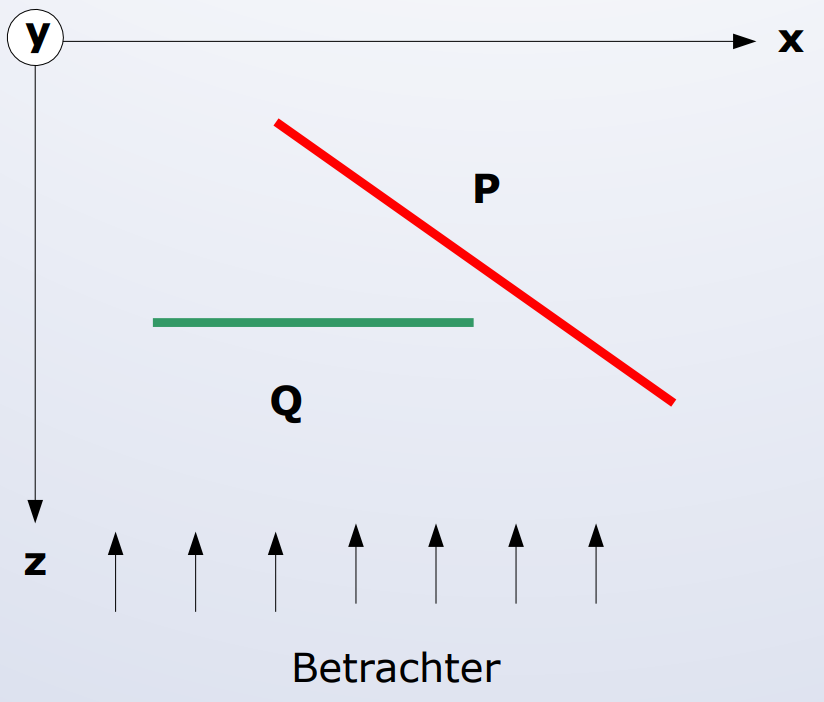
\includegraphics[width=0.15\textwidth]{assets/paintersalg-frontside.png}
  } & \\
  & 4. Liegt Q ganz auf der Betrachterseite  \\
  & von P? (Polygon P ist in der Sortierung \\
  & vor Q) \\
  & \\
  & \\
\end{tabular}

\begin{tabular}{cl}
  \multirow{3}{*}{
    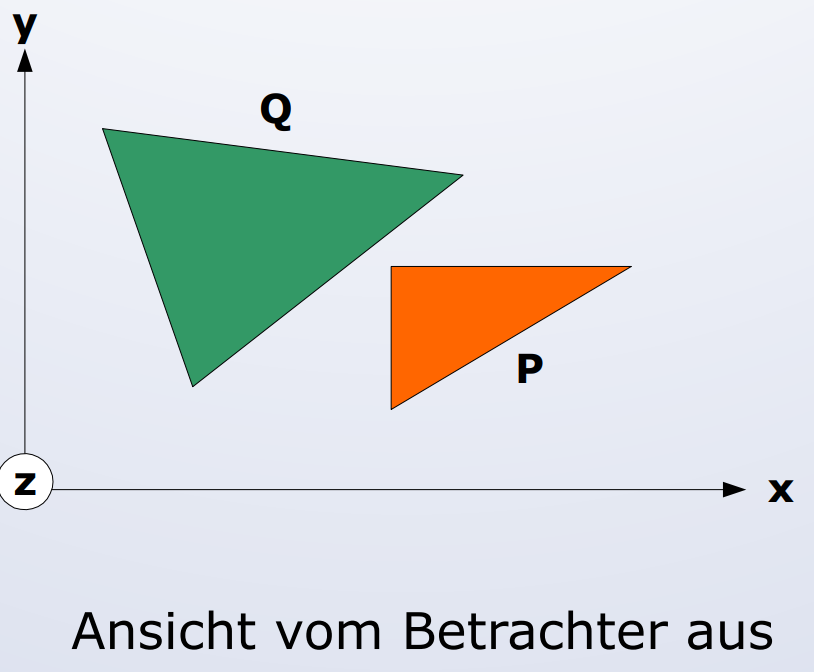
\includegraphics[width=0.15\textwidth]{assets/paintersalg-polygon-overlapping.png}
  } & \\
  & 5. Überlappen sich die Polygone nicht auf \\
  & der Projektion in die xy Ebene? \\
  & \\
  & \\
\end{tabular}

\textit{Bei ungültiger Reihenfolge müssen die Polygone geshnitten werden}

Eigenschaften:
\begin{itemize}
  \item[+] auch für transparente Objekte möglich
  \item[+] einfach für Spezialfälle (2.5D)
  \item[-] ineffizient für viele Objekte O(n2)
  \item[-] nicht Hardware unterstützt
\end{itemize}

\subsection{z-Buffer (WebGL)}
\begin{itemize}
  \item \textit{Pro Pixel Tiefe zusätzlich zur Farbe speichern}
  \item \textit{Beim Zeichnen prüfen, ob näher liegt}
\end{itemize}

\begin{lstlisting}
// Initialisierung
for y = 0 to YMAX do
  for x = 0 to XMAX do
    color[x,y] = Background
    depth[x,y] = MAXDEPTH
  end
end


// Polygone zeichnen
for alle Polygone q do
  for alle pixel p(x,y) in q do
    z = CalculateDepth(q,x,y);
    if z > depth[x,y] then
      depth[x,y] = z;
      color[x,y] = Color of q
    end
  end
end
\end{lstlisting}

Tiefe berechnung aus Ebenegleichung: \\
$z = \frac{-D - Ax - By}{C}$ \\

Inkrementelle Berechnung entlang einer Scanlinie:\\
$Z_{neu} = \frac{-D -A(X_{alt} + 1) - By}{C} = Z_{alt} - \frac{A}{C}$ \\

Eigenschaften:
\begin{itemize}
  \item[+] Hardware unterstützt
  \item[+] Polygone können in beliebiger Reihenfolge gezeichnet werden
  \item[+] Berechenzeit O(n), häufig konstant ab einer gewissen Anzahl Polygone
  \item[-] Rundungsprobleme
  \item[-] Gleiche z-Werte problematisch (Überlagerungsfehler)
  \item[-] (grosser Speicherbedarf)
\end{itemize}

\subsection{Warnock Algorithmus}
\textit{Rekursive Unterteilung des Bildbereichs. Falls "einfach" zu zeichnen -> Zeichnen, sonst unterteilt in 4}\\

\text{Bereich ist zeichenbar wenn:}
\begin{tabular}{cl}
  \multirow{3}{*}{
    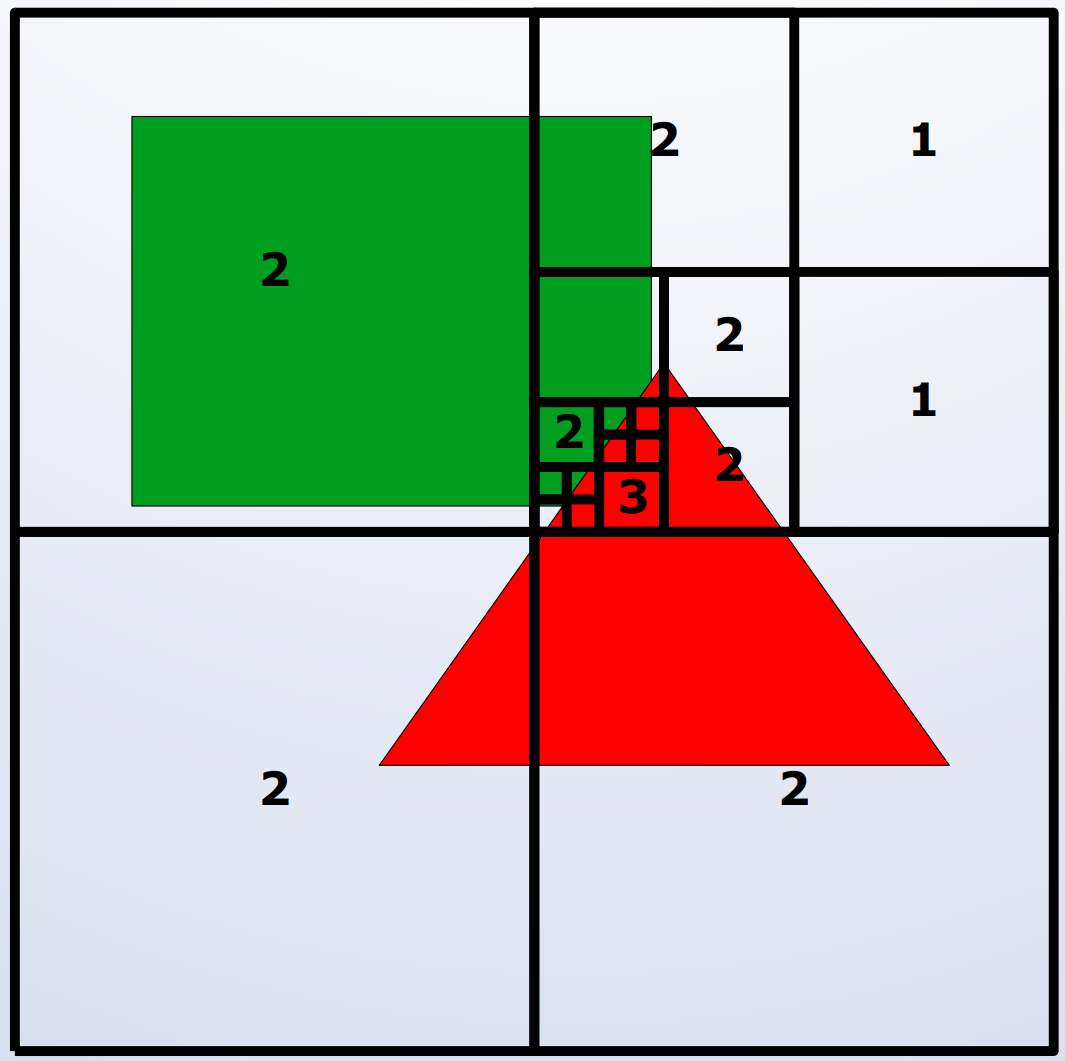
\includegraphics[width=0.2\textwidth]{assets/warnock-alg.png}
  } & - Der Bereich kein Polygon \\
  & enthält \\
  & - Der Bereich nur ein Polygon \\
  & enthält \\
  & - Der Bereich ein Polygon \\
  & enthält, das am nächsten liegt und \\
  & den Bereich vollständig ausfüllt \\
  & - Der Bereich nur aus einem \\
  & Pixel besteht \\
\end{tabular}

\subsection{Objektraum \& Bildraum}

\textit{\textbf{Objektraum} definiert Raum aller Objekte (for alle Objekte)}\\
\textit{\textbf{Bildraum} definiert Raum aller Pixel (for alle Pixel in Bild)}
